\chapter{Obtaining, installing, and validating QMCPACK}
\label{chap:obtaininginstalling}

This chapter describes how to obtain, build, and validate QMCPACK. This process is designed to be as simple as
possible and should be no harder than building a modern plane-wave density
functional theory code such as Quantum ESPRESSO, QBox, or
VASP. Parallel builds enable a complete
compilation in under 2 minutes on a fast multicore system. If you
are unfamiliar with building codes we suggest working with your system
administrator to install QMCPACK.

\section{Installation steps}
To install QMCPACK, follow the steps below. Full details of
each step are given in the referenced sections.
\begin{enumerate}
\item Download the source code (Section~\ref{sec:obrelease} or~\ref{sec:obdevelopment}).
\item Verify that you have the required compilers, libraries, and tools
  installed (Section~\ref{sec:prerequisites}).
\item If you will use Quantum ESPRESSO, download and patch it. The patch adds the
  pw2qmcpack utility (Section~\ref{sec:buildqe}).
\item Run the cmake configure step and build with make (Sections
  \ref{sec:cmake} and~\ref{sec:cmakequick}). Examples for common
  systems are given in Section~\ref{sec:installexamples}.
\item Run the tests to verify QMCPACK (Section~\ref{sec:testing}).
\item Build the ppconvert utility in QMCPACK (Section~\ref{sec:buildppconvert}).
\end{enumerate}

Hints for high performance are in Section~\ref{sec:buildperformance}. Troubleshooting suggestions are in Section~\ref{sec:troubleshoot}.

Note that there are two different QMCPACK executables that can be
produced: the general one, which is the default, and the ``complex''
version, which supports periodic calculations at arbitrary twist angles and
k-points. This second version is enabled via a cmake configuration
parameter (see Section~\ref{sec:cmakeoptions}). The general version
 supports only wavefunctions that can be made real. If you run a
calculation that needs the complex version, QMCPACK will stop and inform you.

\section{Obtaining the latest release version}
\label{sec:obrelease}
Major releases of QMCPACK are distributed from
\url{http://www.qmcpack.org}. Because these versions undergo the most testing, we encourage using them for all production calculations unless there are specific reasons not to do so.

Releases are usually compressed tar files that indicate the version
number, date, and often the source code revision control number
corresponding to the release. To obtain the latest release: 

\begin{itemize}
\item Download the latest QMCPACK distribution from \url{http://www.qmcpack.org}.
\item Untar the archive (e.g., \ishell{tar xvf qmcpack_v1.3.tar.gz}).
\end{itemize}

Releases can also be obtained from the `master' branch of the QMCPACK
git repository, similar to obtaining the development version (Section~\ref{sec:obdevelopment}).

\section{Obtaining the latest development version}
\label{sec:obdevelopment}
The most recent development version of QMCPACK can be obtained anonymously via
\begin{shade}
git clone https://github.com/QMCPACK/qmcpack.git
\end{shade}
Once checked out,
updates can be made via the standard \ishell{git pull}.

The `develop' branch of the git repository contains the day-to-day development source
with the latest updates, bug fixes, etc. This version might be useful
for updates to the build system to support new machines, for support
of the latest versions of Quantum ESPRESSO, or for updates to the
documentation.  Note that the development version might not be fully
consistent with the online documentation.  We attempt to keep
the development version fully working. However, please be sure to run tests and
compare with previous release versions before using for any serious
calculations. We try to keep bugs out, but occasionally they crawl
in! Reports of any breakages are appreciated.

\section{Prerequisites}
\label{sec:prerequisites}
The following items are required to build QMCPACK. For workstations, these are available via the standard
package manager. On shared supercomputers this software is usually
installed by default and is often
accessed via a modules environment---check your system
documentation.

\textbf{Use of the latest versions of all compilers and libraries is
strongly encouraged} but not absolutely essential. Generally, newer versions are faster; see
Section~\ref{sec:buildperformance} for performance suggestions.

\begin{itemize}
\item C/C++ compilers such as GNU, Clang, Intel, and IBM XL. C++ compilers
  are required to support the C++ 14 standard. Use of recent (``current
  year version'') compilers is strongly encouraged.
\item An MPI library such as OpenMPI (\url{http://open-mpi.org}) or a vendor-optimized MPI.
\item BLAS/LAPACK, numerical, and linear algebra libraries. Use
  platform-optimized libraries where available, such as Intel MKL.
  ATLAS or other optimized open source libraries can also be used
  (\url{http://math-atlas.sourceforge.net}).
\item CMake, build utility (\url{http://www.cmake.org}).
\item Libxml2, XML parser (\url{http://xmlsoft.org}).
\item HDF5, portable I/O library (\url{http://www.hdfgroup.org/HDF5/}). Good performance at large scale requires parallel version $>=$ 1.10.
\item BOOST, peer-reviewed portable C++ source libraries  (\url{http://www.boost.org}).   Minimum version is 1.61.0.
\item FFTW, FFT library (\url{http://www.fftw.org/}).
\end{itemize}

To build the GPU accelerated version of QMCPACK, an installation of
NVIDIA CUDA development tools is required. Ensure that this is
compatible with the C and C++ compiler versions you plan to
use. Supported versions are included in the NVIDIA release notes.

Many of the utilities provided with QMCPACK use Python (v2). The numpy
and matplotlib libraries are required for full functionality.

Note that the standalone einspline library used by previous versions of QMCPACK
is no longer required. A more optimized version is included
inside. The standalone version should \emph{not} be on any standard
search paths because conflicts between the old and new include files
can result.

\section{C++ 14 standard library}
The C++ standard consists of language features---which are implemented in the compiler---and library features---which are implemented in the standard library.
GCC includes its own standard library and headers, but many compilers do not and instead reuse those from an existing GCC install.
Depending on setup and installation, some of these compilers might not default to using a GCC with C++ 14 headers (e.g., GCC 4.8 is common as a base system compiler, but its standard library only supports C++ 11).

The symptom of having header files that do not support the C++ 14 standard is usually
compile errors involving standard include header files.
Look for the GCC library version, which should be present in the path to the include file in the error message, and ensure that it is 5.0 or greater.
To avoid these errors occurring at compile time, QMCPACK tests for a C++ 14 standard
library during configuration and will halt with an error if one is not found.

At sites that use modules, running \ishell{module load gcc} is often sufficient to
load a newer GCC and resolve the issue.

\subsection{Intel compiler}
The Intel compiler version must be 18 or newer.
The version 17 compiler cannot compile some of the C++ 14 constructs in the code.

If a newer GCC is needed, the \ishell{-cxxlib} option can be used to point to a different GCC installation.
(Alternately, the \ishell{-gcc-name} or \ishell{-gxx-name} options can be used.)
Be sure to pass this flag to the C compiler in addition to the C++ compiler.
This is necessary because CMake extracts some library paths from the C compiler, and those paths usually also contain to the C++ library.
The symptom of this problem is C++ 14 standard library functions not found at link time.

\section{Building with CMake}
\label{sec:cmake}
The build system for QMCPACK is based on CMake.  It will autoconfigure
based on the detected compilers and libraries. The most recent
version of CMake has the best detection for the greatest variety of
systems.  The minimum required version of CMake is 3.6, which is the
oldest version to support correct application of C++ 14 flags for the Intel compiler.
Most computer installations have a sufficiently recent CMake, though it might not be
the default.

If no appropriate version CMake is available, building it from source is straightforward.
Download a version from \url{https://cmake.org/download/} and unpack the files.
Run \ishell{./boostrap} from the CMake directory, and then run \ishell{make}
when that finishes.  The resulting CMake executable will be in the \ishell{bin/} directory.
The executable can be run directly from that location.

Previously, QMCPACK made extensive use of toolchains, but the build system
has since been updated to eliminate the use of toolchain files for
most cases.  The build system is verified to work with GNU, Intel, and IBM XLC
compilers.  Specific compile options can be specified either through
specific environment or CMake variables.  When the libraries are
installed in standard locations (e.g., /usr, /usr/local), there is no
need to set environment or CMake variables for the packages.

\subsection{Quick build instructions (try first)}
\label{sec:cmakequick}

If you are feeling lucky and are on a standard UNIX-like system such
as a Linux workstation, the following might quickly give a
working QMCPACK:

The safest quick build option is to specify the C and C++ compilers
through their MPI wrappers. Here we use Intel MPI and Intel
compilers. Move to the build directory, run CMake, and make

\begin{shade}
cd build
cmake -DCMAKE_C_COMPILER=mpiicc -DCMAKE_CXX_COMPILER=mpiicpc ..
make -j 8
\end{shade}
You can increase the ``8'' to the number of cores on your system for
faster builds. Substitute mpicc and mpicxx or other wrapped compiler names to suit
  your system. For example, with OpenMPI use

\begin{shade}
cd build
cmake -DCMAKE_C_COMPILER=mpicc -DCMAKE_CXX_COMPILER=mpicxx ..
make -j 8
\end{shade}

If you are feeling particularly lucky, you can skip the compiler specification:

\begin{shade}
cd build
cmake ..
make -j 8
\end{shade}

The complexities of modern computer hardware and software systems are
such that you should check that the autoconfiguration system has made
good choices and picked optimized libraries and compiler settings
before doing significant production. That is, check the following details. We
give examples for a number of common systems in Section~\ref{sec:installexamples}.

\subsection{Environment variables}
\label{sec:envvar}
A number of environment variables affect the build.  In particular
they can control the default paths for libraries, the default
compilers, etc.  The list of environment variables is given below:
%
\begin{shade}
CXX              C++ compiler
CC               C Compiler
MKL_ROOT         Path for MKL
HDF5_ROOT        Path for HDF5
BOOST_ROOT       Path for Boost
FFTW_HOME        Path for FFTW
\end{shade}

\subsection{Configuration options}
\label{sec:cmakeoptions}
In addition to reading the environment variables, CMake provides a
number of optional variables that can be set to control the build and
configure steps.  When passed to CMake, these variables will take
precedent over the environment and default variables.  To set them,
add -D FLAG=VALUE to the configure line between the CMake command and
the path to the source directory.

\begin{itemize}
\item  Key QMCPACK build options
%
\begin{shade}
QMC_CUDA              Enable CUDA and GPU acceleration (1:yes, 0:no)
QMC_COMPLEX           Build the complex (general twist/k-point) version (1:yes, 0:no)
QMC_MIXED_PRECISION   Build the mixed precision (mixing double/float) version
                      (1:yes (GPU default), 0:no (CPU default)).
                      The CPU support is experimental.
                      Use float and double for base and full precision.
                      The GPU support is quite mature.
                      Use always double for host side base and full precision
                      and use float and double for CUDA base and full precision.
ENABLE_SOA            Enable data layout and algorithm optimizations using  
                      Structure-of-Array (SoA) datatypes (1:yes (default), 0:no).  
ENABLE_TIMERS         Enable fine-grained timers (1:yes, 0:no (default)).
                      Timers are off by default to avoid potential slowdown in small
                      systems. For large systems (100+ electrons) there is no risk.
\end{shade}

\item General build options
%
\begin{shade}
CMAKE_BUILD_TYPE     A variable which controls the type of build
                     (defaults to Release). Possible values are:
                     None (Do not set debug/optmize flags, use
                     CMAKE_C_FLAGS or CMAKE_CXX_FLAGS)
                     Debug (create a debug build)
                     Release (create a release/optimized build)
                     RelWithDebInfo (create a release/optimized build with debug info)
                     MinSizeRel (create an executable optimized for size)
CMAKE_C_COMPILER     Set the C compiler
CMAKE_CXX_COMPILER   Set the C++ compiler
CMAKE_C_FLAGS        Set the C flags.  Note: to prevent default
                     debug/release flags from being used, set the CMAKE_BUILD_TYPE=None
                     Also supported: CMAKE_C_FLAGS_DEBUG,
                     CMAKE_C_FLAGS_RELEASE, and CMAKE_C_FLAGS_RELWITHDEBINFO
CMAKE_CXX_FLAGS      Set the C++ flags.  Note: to prevent default
                     debug/release flags from being used, set the CMAKE_BUILD_TYPE=None
                     Also supported: CMAKE_CXX_FLAGS_DEBUG,
                     CMAKE_CXX_FLAGS_RELEASE, and CMAKE_CXX_FLAGS_RELWITHDEBINFO
CMAKE_INSTALL_PREFIX Set the install location (if using the optional install step)
INSTALL_NEXUS        Install Nexus alongside QMCPACK (if using the optional install step)
\end{shade}

\item Additional QMCPACK build options

\begin{shade}
QE_BIN                 Location of Quantum Espresso binaries including pw2qmcpack.x
QMC_DATA               Specify data directory for QMCPACK performance and integration tests
QMC_INCLUDE            Add extra include paths
QMC_EXTRA_LIBS         Add extra link libraries
QMC_BUILD_STATIC       Add -static flags to build
QMC_SYMLINK_TEST_FILES Set to zero to require test files to be copied. Avoids space
                       saving default use of symbolic links for test files. Useful
                       if the build is on a separate filesystem from the source, as
                       required on some HPC systems.
QMC_VERBOSE_CONFIGURATION Print additional information during cmake configuration
                          including details of which tests are enabled.
\end{shade}

\item Intel MKL related
%
\begin{shade}
ENABLE_MKL          Enable Intel MKL libraries (1:yes (default for intel compiler),
                                                0:no (default otherwise)).
MKL_ROOT            Path to MKL libraries (only necessary for non intel compilers
                    or intel without standard environment variables.)
                    One of the above environment variables can be used.
\end{shade}

\item libxml2 related
%
\begin{shade}
LIBXML2_INCLUDE_DIR   Include directory for libxml2
LIBXML2_LIBRARY       Libxml2 library
\end{shade}

\item HDF5 related
%
\begin{shade}
HDF5_PREFER_PARALLEL 1(default for MPI build)/0, enables/disable parallel HDF5 library searching.
ENABLE_PHDF5         1(default for parallel HDF5 library)/0, enables/disable parallel collective I/O.
\end{shade}

\item FFTW related
%
\begin{shade}
FFTW_INCLUDE_DIRS   Specify include directories for FFTW
FFTW_LIBRARY_DIRS   Specify library directories for FFTW
\end{shade}

\item CTest related
%
\begin{shade}
MPIEXEC_EXECUTABLE     Specify the mpi wrapper, e.g. srun, aprun, mpirun, etc.
MPIEXEC_NUMPROC_FLAG   Specify the number of mpi processes flag,
                       e.g. "-n", "-np", etc.
MPIEXEC_PREFLAGS       Flags to pass to MPIEXEC_EXECUTABLE directly before the executable to run.
\end{shade}

\item LLVM/Clang Developer Options\\
\begin{shade}
LLVM_SANITIZE_ADDRESS     link with the %*\href{https://clang.llvm.org/docs/AddressSanitizer.html}{Clang address sanitizer library}*
LLVM_SANITIZE_MEMORY      link with the %*\href{https://clang.llvm.org/docs/MemorySanitizer.html}{Clang memory sanitizer library}*
\end{shade}

See Section~\ref{tool:LLVM-Sanitizer-Libraries} for more information.
\end{itemize}

\subsection{Installation from CMake}
Installation is optional. The QMCPACK executable can be run from the \ishell{bin} directory in the build location.
If the install step is desired, run the \ishell{make install} command to install the QMCPACK executable, the converter,
and some additional executables.
Also installed is the \ishell{qmcpack.settings} file that records options used to compile QMCPACK.
Specify the \ishell{CMAKE_INSTALL_PREFIX} CMake variable during configuration to set the install location.


\subsection{Role of QMC\_DATA}
QMCPACK includes a variety of optional performance and integration
tests that use research quality wavefunctions to obtain meaningful
performance and to more thoroughly test the code. The necessarily
large input files are stored in the location pointed to by QMC\_DATA (e.g., scratch or long-lived project space on a supercomputer). These
files are not included in the source code distribution to minimize
size. The tests are activated if CMake detects the files when
configured. See tests/performance/NiO/README,
tests/solids/NiO\_afqmc/README, tests/performance/C-graphite/README, and tests/performance/C-molecule/README
for details of the current tests and input files and to download them.

Currently the files must be downloaded via \\
\url{https://anl.box.com/s/yxz1ic4kxtdtgpva5hcmlom9ixfl3v3c}.

The layout of current complete set of files is given below. If a file is missing, the appropriate performance test is skipped.
%
\begin{shade}
QMC_DATA/C-graphite/lda.pwscf.h5
QMC_DATA/C-molecule/C12-e48-pp.h5 
QMC_DATA/C-molecule/C12-e72-ae.h5 
QMC_DATA/C-molecule/C18-e108-ae.h5
QMC_DATA/C-molecule/C18-e72-pp.h5 
QMC_DATA/C-molecule/C24-e144-ae.h5
QMC_DATA/C-molecule/C24-e96-pp.h5 
QMC_DATA/C-molecule/C30-e120-pp.h5
QMC_DATA/C-molecule/C30-e180-ae.h5
QMC_DATA/C-molecule/C60-e240-pp.h5
QMC_DATA/NiO/NiO-fcc-supertwist111-supershift000-S1.h5
QMC_DATA/NiO/NiO-fcc-supertwist111-supershift000-S2.h5
QMC_DATA/NiO/NiO-fcc-supertwist111-supershift000-S4.h5
QMC_DATA/NiO/NiO-fcc-supertwist111-supershift000-S8.h5
QMC_DATA/NiO/NiO-fcc-supertwist111-supershift000-S16.h5
QMC_DATA/NiO/NiO-fcc-supertwist111-supershift000-S32.h5
QMC_DATA/NiO/NiO-fcc-supertwist111-supershift000-S64.h5
QMC_DATA/NiO/NiO-fcc-supertwist111-supershift000-S128.h5
QMC_DATA/NiO/NiO-fcc-supertwist111-supershift000-S256.h5
QMC_DATA/NiO/NiO_afm_fcidump.h5
QMC_DATA/NiO/NiO_afm_wfn.dat
QMC_DATA/NiO/NiO_nm_choldump.h5
\end{shade}


\subsection{Configure and build using CMake and make}
To configure and build QMCPACK, move to build directory, run CMake, and make

\begin{shade}
cd build
cmake ..
make -j 8
\end{shade}

As you will have gathered, CMake encourages ``out of source'' builds,
where all the files for a specific build configuration reside in their
own directory separate from the source files. This allows multiple
builds to be created from the same source files, which is very useful
when the file system is shared between different systems. You can also
build versions with different settings (e.g., QMC\_COMPLEX) and
different compiler settings. The build directory does not have to be
called build---use something descriptive such as build\_machinename or
build\_complex. The ``..'' in the CMake line refers to the directory
containing CMakeLists.txt. Update the ``..'' for other build
directory locations.

\subsection{Example configure and build}
\begin{itemize}
\item Set the environments (the examples below assume bash, Intel compilers, and MKL library)

\begin{shade}
export CXX=icpc
export CC=icc
export MKL_ROOT=/usr/local/intel/mkl/10.0.3.020
export HDF5_ROOT=/usr/local
export BOOST_ROOT=/usr/local/boost
export FFTW_HOME=/usr/local/fftw
\end{shade}

\item Move to build directory, run CMake, and make

\begin{shade}
cd build
cmake -D CMAKE_BUILD_TYPE=Release ..
make -j 8
\end{shade}
\end{itemize}

\subsection{Build scripts}
We recommended creating a helper script that contains the
configure line for CMake.  This is particularly useful when avoiding
environment variables, packages are installed in custom locations,
or the configure line is long or complex.  In this case it is also
recommended to add ``rm -rf CMake*" before the configure line to remove
existing CMake configure files to ensure a fresh configure each time
the script is called. Deleting all the files in the build
directory is also acceptable. If you do so we recommend adding some sanity
checks in case the script is run from the wrong directory (e.g.,
checking for the existence of some QMCPACK files).

Some build script examples for different systems are given in the
config directory. For example, on Cray systems these scripts might
load the appropriate modules to set the appropriate programming
environment, specific library versions, etc.

An example script build.sh is given below. It is much more complex
than usually needed for comprehensiveness:


\begin{shade}
export CXX=mpic++
export CC=mpicc
export ACML_HOME=/opt/acml-5.3.1/gfortran64
export HDF5_ROOT=/opt/hdf5
export BOOST_ROOT=/opt/boost

rm -rf CMake*

cmake                                                \
  -D CMAKE_BUILD_TYPE=Debug                         \
  -D LIBXML2_INCLUDE_DIR=/usr/include/libxml2      \
  -D LIBXML2_LIBRARY=/usr/lib/x86_64-linux-gnu/libxml2.so \
  -D FFTW_INCLUDE_DIRS=/usr/include                 \
  -D FFTW_LIBRARY_DIRS=/usr/lib/x86_64-linux-gnu    \
  -D QMC_EXTRA_LIBS="-ldl ${ACML_HOME}/lib/libacml.a -lgfortran" \
  -D QMC_DATA=/projects/QMCPACK/qmc-data            \
  ..
\end{shade}

\subsection{Using vendor-optimized numerical libraries (e.g., Intel MKL})

Although QMC does not make extensive use of linear algebra, use of
vendor-optimized libraries is strongly recommended for highest
performance. BLAS routines are used in the Slater determinant update, the VMC wavefunction optimizer,
and to apply orbital coefficients in local basis calculations. Vectorized
math functions are also beneficial (e.g., for the phase factor
computation in solid-state calculations). CMake is generally successful
in finding these libraries, but specific combinations can require
additional hints, as described in the following:

\subsubsection{Using Intel MKL with non-Intel compilers}

To use Intel MKL with, e.g. an MPICH wrapped gcc:

\begin{shade}
cmake \
 -DCMAKE_C_COMPILER=mpicc -DCMAKE_CXX_COMPILER=mpicxx \
 -DENABLE_MKL=1 -DMKL_ROOT=$MKLROOT/lib \
 ..
\end{shade}

MKLROOT is the directory containing the MKL binary, examples, and lib
directories (etc.) and is often /opt/intel/mkl.

\subsubsection{Serial or multithreaded library}
\label{sec:threadedlibrary}
Vendors might provide both serial and multithreaded versions of their libraries.
Using the right version is critical to QMCPACK performance.
QMCPACK makes calls from both inside and outside threaded regions.
When being called from outside an OpenMP parallel region, the multithreaded version is preferred for the possibility of using all the available cores.
When being called from every thread inside an OpenMP parallel region, the serial version is preferred for not oversubscribing the cores.
Fortunately, nowadays the multithreaded versions of many vendor libraries (MKL, ESSL) are OpenMP aware.
They use only one thread when being called inside an OpenMP parallel region.
This behavior meets exactly both QMCPACK needs and thus is preferred.
If the multithreaded version does not provide this feature of dynamically adjusting the number of threads,
the serial version is preferred. In addition, thread safety is required no matter which version is used.

\subsection{Cross compiling}
Cross compiling is often difficult but is required on supercomputers
with distinct host and compute processor generations or architectures.
QMCPACK tried to do its best with CMake to facilitate cross compiling.

\begin{itemize}
  \item On a machine using a Cray programming environment, we rely on
      compiler wrappers provided by Cray to correctly set architecture-specific
      flags. The CMake configure log should indicate that a
      Cray machine was detected.
  \item If not on a Cray machine, by default we assume building for
    the host architecture (e.g., -xHost is added for the Intel compiler
    and -march=native is added for GNU/Clang compilers).
  \item If -x/-ax or -march is specified by the user in CMAKE\_C\_FLAGS and CMAKE\_CXX\_FLAGS,
    we respect the user's intention and do not add any architecture-specific flags.
\end{itemize}

The general strategy for cross compiling should therefore be to
manually set CMAKE\_C\_FLAGS and CMAKE\_CXX\_FLAGS for the target
architecture. Using \ishell{make VERBOSE=1} is a useful way to check the
final compilation options.  If on a Cray machine, selection of the
appropriate programming environment should be sufficient.

\section{Installation instructions for common workstations and
  supercomputers}
\label{sec:installexamples}

This section describes how to build QMCPACK on various common systems
including multiple Linux distributions, Apple OS X, and various
supercomputers. The examples should serve as good starting points for
building QMCPACK on similar machines. For example, the software
environment on modern Crays is very consistent. Note that updates to
operating systems and system software might require small modifications
to these recipes. See Section~\ref{sec:buildperformance} for key
points to check to obtain highest performance and
Section~\ref{sec:troubleshoot} for troubleshooting hints.

\subsection{Installing on Ubuntu Linux or other apt-get--based distributions}
\label{sec:buildubuntu}

The following is designed to obtain a working QMCPACK build on, for example, a
student laptop, starting from a basic Linux installation with none of
the developer tools installed. Fortunately, all the required packages
are available in the default repositories making for a quick
installation. Note that for convenience we use a generic BLAS. For
production, a platform-optimized BLAS should be used.

\begin{shade}
apt-get cmake g++ openmpi-bin libopenmpi-dev libboost-dev
apt-get libatlas-base-dev liblapack-dev libhdf5-dev libxml2-dev fftw3-dev
export CXX=mpiCC
cd build
cmake ..
make -j 8
ls -l bin/qmcpack
\end{shade}

For qmca and other tools to function, we install some Python libraries:

\begin{shade}
sudo apt-get install python-numpy python-matplotlib
\end{shade}

\subsection{Installing on CentOS Linux or other yum-based distributions}

The following is designed to obtain a working QMCPACK build on, for example, a
student laptop, starting from a basic Linux installation with none of
the developer tools installed. CentOS 7 (Red Hat compatible) is using
gcc 4.8.2. The installation is complicated only by the need to install
another repository to obtain HDF5 packages that are not available by
default. Note that for convenience we use a generic BLAS. For
production, a platform-optimized BLAS should be used.

\begin{shade}
sudo yum install make cmake gcc gcc-c++ openmpi openmpi-devel fftw fftw-devel \
                  boost boost-devel libxml2 libxml2-devel
sudo yum install blas-devel lapack-devel atlas-devel
module load mpi
\end{shade}

To setup repoforge as a source for the HDF5 package, go to
\url{http://repoforge.org/use}. Install the appropriate up-to-date
release package for your operating system. By default, CentOS Firefox will offer
to run the installer. The CentOS 6.5 settings were still usable for HDF5 on
CentOS 7 in 2016, but use CentOS 7 versions when they become
available.


\begin{shade}
sudo yum install hdf5 hdf5-devel
\end{shade}

To build QMCPACK:

\begin{shade}
module load mpi/openmpi-x86_64
which mpirun
# Sanity check; should print something like   /usr/lib64/openmpi/bin/mpirun
export CXX=mpiCC
cd build
cmake ..
make -j 8
ls -l bin/qmcpack
\end{shade}

\subsection{Installing on Mac OS X using Macports}
These instructions assume a fresh installation of macports
and use the gcc 6.1 compiler. Older versions are fine, but it is vital to ensure that 
matching compilers and libraries are used for all
packages and to force use of what is installed in /opt/local.  Performance should be very reasonable.
Note that we use the Apple-provided Accelerate framework for
optimized BLAS.

Follow the Macports install instructions at \url{https://www.macports.org/}.

\begin{itemize}
\item Install Xcode and the Xcode Command Line Tools.
\item Agree to Xcode license in Terminal: sudo xcodebuild -license.
\item Install MacPorts for your version of OS X.
\end{itemize}

Install the required tools:

\begin{shade}
sudo port install gcc6
sudo port select gcc mp-gcc6
sudo port install openmpi-devel-gcc6
sudo port select --set mpi openmpi-devel-gcc61-fortran

sudo port install fftw-3 +gcc6
sudo port install libxml2
sudo port install cmake
sudo post install boost +gcc6
sudo port install hdf5 +gcc6

sudo port select --set python python27
sudo port install py27-numpy +gcc6
sudo port install py27-matplotlib  #For graphical plots with qmca
\end{shade}

QMCPACK build:

\begin{shade}
cd build
cmake -DCMAKE_C_COMPILER=mpicc -DCMAKE_CXX_COMPILER=mpiCXX ..
make -j 6 # Adjust for available core count
ls -l bin/qmcpack
\end{shade}

Cmake should pickup the versions of HDF5 and libxml (etc.) installed in
/opt/local by macports. If you have other copies of these libraries
installed and wish to force use of a specific version, use the
environment variables detailed in Section~\ref{sec:envvar}.

This recipe was verified on July 1, 2016, on a Mac running OS X 10.11.5
``El Capitain.''

\subsection{Installing on Mac OS X using Homebrew (brew)}
Homebrew is a package manager for OS X that provides a convenient
route to install all the QMCPACK dependencies. The
following recipe will install the latest available versions of each
package. This was successfully tested under OS X 10.12 ``Sierra'' in December 2017. Note that it is necessary to build the MPI software from
source to use the brew-provided gcc instead of Apple CLANG.

\begin{enumerate}
\item Install Homebrew from \url{http://brew.sh/}:
%
\begin{shade}
/usr/bin/ruby -e "$(curl -fsSL
    https://raw.githubusercontent.com/Homebrew/install/master/install)"
\end{shade}
 
\item Install the prerequisites:
%
\begin{shade}
brew install gcc # installs gcc 7.2.0 on 2017-12-19
export HOMEBREW_CXX=g++-7
export HOMEBREW_CC=gcc-7
brew install mpich2 --build-from-source
# Build from source required to use homebrew compiled compilers as
# opposed to Apple CLANG. Check "mpicc -v" indicates Homebrew gcc
brew install cmake
brew install fftw
brew install boost
brew install homebrew/science/hdf5
#Note: Libxml2 is not required via brew since OS X already includes it.
\end{shade}
\item Configure and build QMCPACK:
%
\begin{shade}
cmake -DCMAKE_C_COMPILER=/usr/local/bin/mpicc \
      -DCMAKE_CXX_COMPILER=/usr/local/bin/mpicxx ..
make -j 12
\end{shade}
\item Run the short tests. When MPICH is used for the first time, OS
  X will request approval of the network connection for each executable.
%
\begin{shade}
ctest -R short -LE unstable
\end{shade}
\end{enumerate}

\subsection{Installing on ALCF Theta, Cray XC40}
Theta is a 9.65 petaflops system manufactured by Cray with 3,624 compute nodes.
Each node features a second-generation Intel Xeon Phi 7230 processor and 192 GB DDR4 RAM.

%
\begin{shade}
export CRAYPE_LINK_TYPE=dynamic
# Do not use cmake 3.9.1, it causes trouble with parallel HDF5.
module load cmake/3.11.4
module unload cray-libsci
module load cray-hdf5-parallel
module load gcc   # Make C++ 14 standard library available to the Intel compiler
export BOOST_ROOT=/soft/libraries/boost/1.64.0/intel
cmake ..
make -j 24
ls -l bin/qmcpack
\end{shade}

\subsection{Installing on ORNL OLCF Summit}
Summit is an IBM system at the ORNL OLCF built with IBM Power System AC922
nodes. They have two IBM Power 9 processors and six NVIDIA Volta V100
accelerators.

\subsubsection{Building QMCPACK}
Note that these build instructions are preliminary as the
software environment is subject to change. As of December 2018, the
IBM XL compiler does not support C++14, so we currently use the
gnu compiler. 

For ease of reproducibility we provide build scripts for summit.
\lstset{language=bash,style=SHELL}
\begin{lstlisting}
cd qmcpack
./config/build_olcf_summit.sh
ls bin
\end{lstlisting}

\subsubsection{Building Quantum Espresso}
We provide a build script for the v6.4.1 release of Quantum Espresso (QE).
The following can be used to build a CPU version of QE on Summit,
placing the script in the external\_codes/quantum\_espresso directory.

\begin{lstlisting}
cd external_codes/quantum_espresso
./build_qe_olcf_summit.sh
\end{lstlisting}

Note that performance is
not yet optimized although vendor libraries are
used. Alternatively, the wavefunction files can be generated on
another system and the converted HDF5 files copied over.

\subsection{Installing on NERSC Cori, Haswell Partition, Cray XC40}
Cori is a Cray XC40 that includes 16-core Intel "Haswell" nodes
installed at NERSC. In the following example, the source code is
cloned in \$HOME/qmc/git\_QMCPACK and QMCPACK is built in the scratch
space.

\begin{shade}
mkdir $HOME/qmc
mkdir $HOME/qmc/git_QMCPACK
cd $HOME/qmc_git_QMCPACK
git clone https://github.com/QMCPACK/qmcpack.git
cd qmcpack
git checkout v3.7.0 # Edit for desired version
export CRAYPE_LINK_TYPE=dynamic
module unload cray-libsci
module load boost/1.70.0
module load cray-hdf5-parallel
module load cmake/3.14.0
module load gcc/7.3.0 # Make C++ 14 standard library available to the Intel compiler
cd $SCRATCH
mkdir build_cori_hsw
cd build_cori_hsw
cmake -DQMC_SYMLINK_TEST_FILES=0 $HOME/qmc/git_QMCPACK/qmcpack/
nice make -j 8
ls -l bin/qmcpack
\end{shade}

When the preceding was tested on May 16, 2019, the following module and
software versions were present:

\begin{shade}
build_cori_hsw> module list
Currently Loaded Modulefiles:
  1) modules/3.2.10.6                                 14) alps/6.6.43-6.0.7.1_5.45__ga796da32.ari
  2) nsg/1.2.0                                        15) rca/2.2.18-6.0.7.1_5.47__g2aa4f39.ari
  3) intel/18.0.1.163                                 16) atp/2.1.3
  4) craype-network-aries                             17) PrgEnv-intel/6.0.4
  5) craype/2.5.15                                    18) craype-haswell
  6) udreg/2.3.2-6.0.7.1_5.13__g5196236.ari           19) cray-mpich/7.7.3
  7) ugni/6.0.14.0-6.0.7.1_3.13__gea11d3d.ari         20) gcc/7.3.0
  8) pmi/5.0.14                                       21) altd/2.0
  9) dmapp/7.1.1-6.0.7.1_5.45__g5a674e0.ari           22) darshan/3.1.4
 10) gni-headers/5.0.12.0-6.0.7.1_3.11__g3b1768f.ari  23) boost/1.70.0
 11) xpmem/2.2.15-6.0.7.1_5.11__g7549d06.ari          24) cray-hdf5-parallel/1.10.2.0
 12) job/2.2.3-6.0.7.1_5.43__g6c4e934.ari             25) cmake/3.14.0
 13) dvs/2.7_2.2.118-6.0.7.1_10.1__g58b37a2
\end{shade}

To following slurm job file can be used to run the tests:
\begin{shade}
#!/bin/bash
#SBATCH --qos=debug
#SBATCH --time=00:10:00
#SBATCH --nodes=1
#SBATCH --tasks-per-node=32
#SBATCH --constraint=haswell
echo --- Start `date` 
echo --- Working directory: `pwd`
ctest -VV -R deterministic
echo --- End `date`
\end{shade}

\subsection{Installing on NERSC Cori, Xeon Phi KNL partition, Cray XC40}
Cori is a Cray XC40 that includes Intel Xeon Phi Knight's Landing (KNL) nodes. The following build recipe ensures that the code
generation is appropriate for the KNL nodes. The source is assumed to
be in \$HOME/qmc/git\_QMCPACK/qmcpack as per the Haswell example.

\begin{shade}
export CRAYPE_LINK_TYPE=dynamic
module swap craype-haswell craype-mic-knl # Only difference between Haswell and KNL recipes
module unload cray-libsci
module load boost/1.70.0
module load cray-hdf5-parallel
module load cmake/3.14.0
module load gcc/7.3.0 # Make C++ 14 standard library available to the Intel compiler
cd $SCRATCH
mkdir build_cori_knl
cd build_cori_knl
cmake -DQMC_SYMLINK_TEST_FILES=0 $HOME/git_QMCPACK/qmcpack/
nice make -j 8
ls -l bin/qmcpack
\end{shade}

When the preceding was tested on May 16, 2019, the following module and
software versions were present:

\begin{shade}
build_cori_knl> module list
  Currently Loaded Modulefiles:
  1) modules/3.2.10.6                                 14) alps/6.6.43-6.0.7.1_5.45__ga796da32.ari
  2) nsg/1.2.0                                        15) rca/2.2.18-6.0.7.1_5.47__g2aa4f39.ari
  3) intel/18.0.1.163                                 16) atp/2.1.3
  4) craype-network-aries                             17) PrgEnv-intel/6.0.4
  5) craype/2.5.15                                    18) craype-mic-knl
  6) udreg/2.3.2-6.0.7.1_5.13__g5196236.ari           19) cray-mpich/7.7.3
  7) ugni/6.0.14.0-6.0.7.1_3.13__gea11d3d.ari         20) gcc/7.3.0
  8) pmi/5.0.14                                       21) altd/2.0
  9) dmapp/7.1.1-6.0.7.1_5.45__g5a674e0.ari           22) darshan/3.1.4
 10) gni-headers/5.0.12.0-6.0.7.1_3.11__g3b1768f.ari  23) boost/1.70.0
 11) xpmem/2.2.15-6.0.7.1_5.11__g7549d06.ari          24) cray-hdf5-parallel/1.10.2.0
 12) job/2.2.3-6.0.7.1_5.43__g6c4e934.ari             25) cmake/3.14.0
 13) dvs/2.7_2.2.118-6.0.7.1_10.1__g58b37a2
\end{shade}

\subsection{Installing on systems with ARMv8-based processors}
The following build recipe was verified using the `Arm Compiler for HPC' on the ANL JLSE Comanche system with Cavium ThunderX2 processors on November 6, 2018.
\begin{shade}
# load armclang compiler
module load Generic-AArch64/RHEL/7/arm-hpc-compiler/18.4
# load Arm performance libraries
module load ThunderX2CN99/RHEL/7/arm-hpc-compiler-18.4/armpl/18.4.0
# define path to pre-installed packages
export HDF5_ROOT=</path/to/hdf5/install/>
export BOOST_ROOT=</path/to/boost/install> # header-only, no need to build
\end{shade}
Then using the following command:
\begin{shade}
mkdir build_armclang
cd build_armclang
cmake -DCMAKE_C_COMPILER=armclang -DCMAKE_CXX_COMPILER=armclang++ -DQMC_MPI=0 \
      -DLAPACK_LIBRARIES="-L$ARMPL_DIR/lib -larmpl_mp" \
      -DFFTW_INCLUDE_DIR="$ARMPL_DIR/include" \
      -DFFTW_LIBRARIES="$ARMPL_DIR/lib/libarmpl_mp.a" \
      ..
make -j 56
\end{shade}
Note that armclang is recognized as an `unknown' compiler by CMake v3.13* and below. In this case, we need to force it as clang to apply necessary flags. To do so, pass the following additionals option to CMake:
\begin{shade}
      -DCMAKE_C_COMPILER_ID=Clang -DCMAKE_CXX_COMPILER_ID=Clang \
      -DCMAKE_CXX_COMPILER_VERSION=5.0 -DCMAKE_CXX_STANDARD_COMPUTED_DEFAULT=98 \
\end{shade}      

\subsection{Installing on Windows}
Install the Windows Subsystem for Linux and Bash on Windows.
Open a bash shell and follow the install directions for Ubuntu in Section~\ref{sec:buildubuntu}.

\section{Installing via Spack}
Spack is a package manager for scientific software.  One of the
primary goals of Spack is to reduce the barrier for users to install
scientific software. Spack is intended to work on everything from
laptop computers to high-end supercomputers. More information about
Spack can be found at
\url{https://spack.readthedocs.io/en/latest}. The major advantage of
installation with Spack is that all dependencies are automatically
built, potentially including all the compilers and libraries, and
different versions of QMCPACK can easily coexist with each other. We
are also able to install a patched version of Quantum ESPRESSO (QE)
via a seperate Spack command. Earlier versions of the QMCPACK Spack
package bundled QE as a variant, but this method was not robust and
frequently led to installation failures.

With a properly configured Spack environment, you can be up and
running on your computer with two simple commaneds:
\begin{shade}
your-laptop> spack install qmcpack@3.9.2%gcc

your-laptop> spack install quantum-espresso+qmcpack~patch@6.4.1%gcc hdf5=parallel
\end{shade}

A more detailed explanation of these commands and the syntax follows.


\subsection{Known Limitations}
The QMCPACK Spack package inherits the limitations of the underlying
Spack infrastructure and its dependencies. The main limitation is that
installation can fail when building a dependency such as HDF5, MPICH,
etc. For \ishell{spack install qmcpack} to succeed, it is very
important to leverage preinstalled packages on your computer or
supercomputer. The other frequently encountered challenge is that the
compiler configuration is nonintuitive.  This is especially the case
with the Intel compiler. If you encounter any difficulties, we
recommend testing the Spack compiler configuration on a simpler
packages, e.g. HDF5.

Here are some additional limitations of the QMCPACK Spack package that
will be resolved in future releases:
\begin{itemize}
\item CUDA support in Spack still has some limitations.  It will
  catch only some compiler-CUDA conflicts.
\item The Intel compiler must find a recent and compatible GCC
  compiler in its path or one must be explicity set with the
  \ishell{-gcc-name} and \ishell{-gxx-name} flags.
\end{itemize}

\subsection{Setting up the Spack Environment}
Begin by cloning Spack from GitHub and configuring your shell as described at 
\url{https://spack.readthedocs.io/en/latest/getting_started.html}.

The goal of the next several steps is to set up the Spack environment
for building. First, we highly recommend limiting the number of build jobs to
a reasonable value for your machine. This can be
accomplished by modifying your \ishell{\~/.spack/config.yaml} file as follows:

\begin{lstlisting}[style=SHELL]
config:
  build_jobs: 16
\end{lstlisting}

Make sure any existing compilers are properly detected. For many
architectures, compilers are properly detected with no additional
effort.

\begin{shade}
your-laptop> spack compilers
==> Available compilers
-- gcc sierra-x86_64 --------------------------------------------
gcc@7.2.0  gcc@6.4.0  gcc@5.5.0  gcc@4.9.4  gcc@4.8.5  gcc@4.7.4  gcc@4.6.4
\end{shade}

However, if your compiler is not automatically detected, it is straightforward
to add one:

\begin{shade}
your-laptop> spack compiler add <path-to-compiler>
\end{shade}

The Intel compiler, and other commerical compilers like PGI, typically
require extra environment variables to work properly. If you have an
module environment set-up by your system administrators, it is
recommended that you set the module name in
\ishell{\~/.spack/linux/compilers.yaml}. Here is an example for the
Intel compiler
\begin{shade}
- compiler:
    environment:{}
    extra_rpaths:  []
    flags: {}
    modules:
    - intel/18.0.3
    operating_system: ubuntu14.04
    paths:
      cc: /soft/com/packages/intel/18/u3/compilers_and_libraries_2018.3.222/linux/bin/intel64/icc
      cxx: /soft/com/packages/intel/18/u3/compilers_and_libraries_2018.3.222/linux/bin/intel64/icpc
      f77: /soft/com/packages/intel/18/u3/compilers_and_libraries_2018.3.222/linux/bin/intel64/ifort
      fc: /soft/com/packages/intel/18/u3/compilers_and_libraries_2018.3.222/linux/bin/intel64/ifort
    spec: intel@18.0.3
    target: x86_64
\end{shade}

If a module is not available, you will have to set-up the environment variables manually:
\begin{shade}
- compiler:
    environment:
      set:
        INTEL_LICENSE_FILE: server@national-lab.doe.gov
    extra_rpaths:  ['/soft/com/packages/intel/18/u3/compilers_and_libraries_2018.3.222/linux/compiler/lib/intel64',
    '/soft/apps/packages/gcc/gcc-6.2.0/lib64']
    flags: 
      cflags: -gcc-name=/soft/apps/packages/gcc/gcc-6.2.0/bin/gcc
      fflags: -gcc-name=/soft/apps/packages/gcc/gcc-6.2.0/bin/gcc
      cxxflags: -gxx-name=/soft/apps/packages/gcc/gcc-6.2.0/bin/g++
    modules: []
    operating_system: ubuntu14.04
    paths:
      cc: /soft/com/packages/intel/18/u3/compilers_and_libraries_2018.3.222/linux/bin/intel64/icc
      cxx: /soft/com/packages/intel/18/u3/compilers_and_libraries_2018.3.222/linux/bin/intel64/icpc
      f77: /soft/com/packages/intel/18/u3/compilers_and_libraries_2018.3.222/linux/bin/intel64/ifort
      fc: /soft/com/packages/intel/18/u3/compilers_and_libraries_2018.3.222/linux/bin/intel64/ifort
    spec: intel@18.0.3
    target: x86_64
\end{shade}

This last step is the most troublesome. Pre-installed packages are not
automatically detected. If vendor optimized libraries are already
installed, you will need to manually add them to your
\ishell{\~/.spack/packages.yaml}. For example, this works on Mac OS X
for the Intel MKL package.

\begin{shade}
your-laptop> cat ~/.spack/packages.yaml
packages:
    intel-mkl:
        paths:
            intel-mkl@2018.0.128: /opt/intel/compilers_and_libraries_2018.0.104/mac/mkl
        buildable: False
\end{shade}

Some trial-and-error might be involved to set the directories
correctly. If you do not include enough of the tree path, Spack will
not be able to register the package in its database. More information
about system packages can be found at
\url{http://spack.readthedocs.io/en/latest/getting_started.html#system-packages}

Beginning with QMCPACK v3.9.0, Python 3.x is required. However,
installing Python with a compiler besides GCC is tricky. We recommend
leveraging your local Python installation by adding an entry in
\ishell{\~/.spack/packages.yaml}:
\begin{shade}
packages:
    python:
       modules:
         python@3.7.4: anaconda3/2019.10
\end{shade}

Or if a module is not available
\begin{shade}
packages:
    python:
       paths:
          python@3.7.4: /nfs/gce/software/custom/linux-ubuntu18.04-x86_64/anaconda3/2019.10/bin/python
       buildable: False
\end{shade}


\subsection{Building QMCPACK}
The QMCPACK Spack package has a number of variants to support different compile time
options and different versions of the application. A full list can be displayed by typing:

\begin{lstlisting}[style=SHELL]
your laptop> spack info qmcpack
CMakePackage:   qmcpack

Description:
    QMCPACK, is a modern high-performance open-source Quantum Monte Carlo
    (QMC) simulation code.

Homepage: http://www.qmcpack.org/

Tags: 
    ecp  ecp-apps

Preferred version:  
    3.9.2      [git] https://github.com/QMCPACK/qmcpack.git at tag v3.9.2

Safe versions:  
    develop  [git] https://github.com/QMCPACK/qmcpack.git
    3.9.2      [git] https://github.com/QMCPACK/qmcpack.git at tag v3.9.2
    3.9.1      [git] https://github.com/QMCPACK/qmcpack.git at tag v3.9.1
    3.9.0      [git] https://github.com/QMCPACK/qmcpack.git at tag v3.9.0
    3.8.0      [git] https://github.com/QMCPACK/qmcpack.git at tag v3.8.0
    3.7.0      [git] https://github.com/QMCPACK/qmcpack.git at tag v3.7.0
    3.6.0      [git] https://github.com/QMCPACK/qmcpack.git at tag v3.6.0
    3.5.0      [git] https://github.com/QMCPACK/qmcpack.git at tag v3.5.0
    3.4.0      [git] https://github.com/QMCPACK/qmcpack.git at tag v3.4.0
    3.3.0      [git] https://github.com/QMCPACK/qmcpack.git at tag v3.3.0
    3.2.0      [git] https://github.com/QMCPACK/qmcpack.git at tag v3.2.0
    3.1.1      [git] https://github.com/QMCPACK/qmcpack.git at tag v3.1.1
    3.1.0      [git] https://github.com/QMCPACK/qmcpack.git at tag v3.1.0

Variants:
    Name [Default]          Allowed values          Description
    ====================    ====================    ====================
    afqmc [off]             True, False             Install with AFQMC support.
                                                    NOTE that if used in
                                                    combination with CUDA, only
                                                    AFQMC will have CUDA.
    build_type [Release]    Debug, Release,         The build type to build
                            RelWithDebInfo
    complex [off]           True, False             Build the complex (general
                                                    twist/k-point) version
    cuda [off]              True, False             Build with CUDA
    cuda_arch [none]        none, 53, 20, 62,       CUDA architecture
                            60, 61, 50, 75, 70,     
                            72, 32, 52, 30, 35      
    da [off]                True, False             Install with support for basic
                                                    data analysis tools
    gui [off]               True, False             Install with Matplotlib (long
                                                    installation time)
    mixed [off]             True, False             Build the mixed precision
                                                    (mixture of single and double
                                                    precision) version for gpu and
                                                    cpu
    mpi [on]                True, False             Build with MPI support
    phdf5 [on]              True, False             Build with parallel collective
                                                    I/O
    ppconvert [off]         True, False             Install with pseudopotential
                                                    converter.
    soa [on]                True, False             Build with Structure-of-Array
                                                    instead of Array-of-Structure
                                                    code. Only for CPU codeand
                                                    only in mixed precision
    timers [off]            True, False             Build with support for timers

Installation Phases:
    cmake    build    install

Build Dependencies:
    blas  boost  cmake  cuda  fftw-api  hdf5  lapack  libxml2  mpi  python

Link Dependencies:
    blas  boost  cuda  fftw-api  hdf5  lapack  libxml2  mpi  python

Run Dependencies:
    py-matplotlib  py-numpy  quantum-espresso

Virtual Packages: 
    None
\end{lstlisting}

For example, to install the complex-valued version of QMCPACK in mixed-precision use:

\begin{shade}
your-laptop> spack install qmcpack+mixed+complex%gcc@7.2.0 ^intel-mkl
\end{shade}
where the \ishell{+} decorators in front of \ishell{mixed} and
\ishell{complex} indicate that the variant should be activated.

\begin{shade}
%gcc@7.2.0
\end{shade}
specifies the compiler version to be used and

\begin{shade}
^intel-mkl
\end{shade}
specifies that the Intel MKL should be used as the BLAS and LAPACK
provider. The \ishell{^} symbol indicates the the package to the right of the
symbol should be used to fulfill the dependency needed by the installation.

It is also possible to run the QMCPACK regression tests as part of the
installation process, for example:

\begin{shade}
your-laptop> spack install --test=root qmcpack+mixed+complex%gcc@7.2.0 ^intel-mkl
\end{shade}
will run the unit and short tests. The current behavior of the QMCPACK
Spack package is to complete the install as long as all the unit tests
pass. If the short tests fail, a warning is issued at the command prompt.

For CUDA, you will need to specify and extra \ishell{cuda_arch}
parameter otherwise, it will default to \ishell{cuda_arch=61}.
\begin{shade}
your-laptop> spack install qmcpack+cuda%intel@18.0.3 cuda_arch=61 ^intel-mkl
\end{shade}

Due to limitations in the Spack CUDA package, if your compiler and
CUDA combination conflict, you will need to set a
specific verison of CUDA that is compatible with your compiler on the
command line. For example,
\begin{shade}
your-laptop> spack install qmcpack+cuda%intel@18.0.3 cuda_arch=61 ^cuda@10.0.130 ^intel-mkl
\end{shade}

\subsection{Loading QMCPACK into your environment}
If you already have modules set-up in your enviroment, the Spack
modules will be detected automatically. Otherwise, Spack will not
automatically find the additional packages. A few additional steps are
needed.  Please see the main Spack documentation for additional details:
\url{https://spack.readthedocs.io/en/latest/module_file_support.html}

\subsection{Dependencies that need to be compiled with GCC}
Failing to compile a QMCPACK dependency is the most common reason that
a Spack build fails. We recommend that you compile the following
dependencies with GCC:

For MPI, using MPICH as the provider, try:
\begin{shade}

your-laptop> spack install qmcpack%intel@18.0.3 ^boost%gcc ^pkgconf%gcc ^perl%gcc ^libpciaccess%gcc ^cmake%gcc ^findutils%gcc ^m4%gcc
\end{shade}

For serial,
\begin{shade}

your-laptop> spack install qmcpack~mpi%intel@18.0.3 ^boost%gcc ^pkgconf%gcc ^perl%gcc ^cmake%gcc

\end{shade}

\subsection{Installing QMCPACK with Spack on Linux}
Spack works robustly on the standard flavors of Linux (Ubuntu, CentOS,
Ubuntu, etc.) using GCC, Clang, PGI, and Intel compilers.

\subsection{Installing QMCPACK with Spack on Mac OS X}
Spack works on Mac OS X but requires installation of a few packages
using Homebrew. You will need to install at minimum the GCC compilers,
CMake, and pkg-config. The Intel compiler for Mac on OS X is not well
supported by Spack packages and will most likely lead to a compile
time failure in one of QMCPACK's dependencies.

\subsection{Installing QMCPACK with Spack on Cray Supercomputers}
Spack now works with the Cray environment. To leverage the installed
Cray environment, both a \ishell{compilers.yaml} and
\ishell{packages.yaml} file should be provided by the supercomputing
facility. Additionally, Spack packages compiled by the facility can be
reused by chaining Spack installations
\url{https://spack.readthedocs.io/en/latest/chain.html}

Instructions for DOE supercomputing facilities that support Spack directly will be forthcoming.

\subsection{Reporting Bugs}
Bugs with the QMCPACK Spack package should be filed at the main GitHub
Spack repo \url{https://github.com/spack/spack/issues}

In the GitHub issue, include \ishell{@naromero77} to get the attention
of our developer.

\section{Testing and validation of QMCPACK}
\label{sec:testing}
We \textbf{strongly encourage} running the included tests each time
QMCPACK is built. A range of unit and integration tests ensure that
the code behaves as expected and that results are consistent with
known-good mean-field, quantum chemical, and historical QMC results.

The tests include the following:
\begin{itemize}
\item Unit tests: to check fundamental behavior. These should always pass.
\item Stochastic integration tests: to check computed results from
  the Monte Carlo methods. These might fail statistically, but rarely
  because of the use of three sigma level statistics. These tests are
  further split into ``short'' tests, which have just sufficient
  length to have valid statistics, and ``long'' tests, to check
  behavior to higher statistical accuracy.
\item Converter tests: to check conversion of trial wavefunctions
  from codes such as QE and GAMESS to QMCPACK's
  formats. These should always pass.
\item Workflow tests: in the case of QE, we test the
  entire cycle of DFT calculation, trial wavefunction conversion, and
  a subsequent VMC run.  
\item Performance: to help performance monitoring. Only the timing of
  these runs is relevant.  
\end{itemize}


The test types are differentiated by prefixes in their names, for example, \ishell{short-LiH_dimer_ae_vmc_hf_noj_16-1} indicates a short VMC test
for the LiH dime. 

QMCPACK also includes tests for developmental features and features
that are unsupported on certain platforms. To indicate these, tests
that are unstable are labeled with the CTest label
``unstable.'' For example, they are unreliable, unsupported, or known to fail
from partial implementation or bugs.

When installing QMCPACK you should run at least the unit tests:

\begin{shade}
 ctest -R unit
 \end{shade}
 
These tests take only a few seconds to run. All should pass. A
failure here could indicate a major problem with the installation.

A wider range of deterministic integration
tests are being developed. The goal is to test much more of QMCPACK than the unit tests
do and to do so in a manner that is reproducible
across platforms. All of these should eventually pass 100\% reliably
and quickly. At present, some fail on some platforms and for certain
build types.

 \begin{shade}
 ctest -R deterministic -LE unstable
 \end{shade}

If time allows, the ``short'' stochastic tests should also be run.
The short tests take a few minutes each on a 16-core machine---about 1 hour total depending on the platform. You can run these tests using the following command in the
build directory:


\begin{shade}
ctest -R short -LE unstable  # Run the tests with "short" in their name.
                             # Exclude any known unstable tests.
\end{shade}
The output should be similar to the following:

\begin{shade}
Test project build_gcc
      Start  1: short-LiH_dimer_ae-vmc_hf_noj-16-1
 1/44 Test  #1: short-LiH_dimer_ae-vmc_hf_noj-16-1 ..............  Passed   11.20 sec
      Start  2: short-LiH_dimer_ae-vmc_hf_noj-16-1-kinetic
 2/44 Test  #2: short-LiH_dimer_ae-vmc_hf_noj-16-1-kinetic ......  Passed    0.13 sec
..
42/44 Test #42: short-monoO_1x1x1_pp-vmc_sdj-1-16 ...............  Passed   10.02 sec
      Start 43: short-monoO_1x1x1_pp-vmc_sdj-1-16-totenergy
43/44 Test #43: short-monoO_1x1x1_pp-vmc_sdj-1-16-totenergy .....  Passed    0.08 sec
      Start 44: short-monoO_1x1x1_pp-vmc_sdj-1-16-samples
44/44 Test #44: short-monoO_1x1x1_pp-vmc_sdj-1-16-samples .......  Passed    0.08 sec

100% tests passed, 0 tests failed out of 44

Total Test time (real) = 167.14 sec
\end{shade}

Note that the number of tests run varies between the
standard, complex, and GPU compilations. These tests should pass with three sigma reliability. That is, they should nearly always pass, and when rerunning a failed test it should usually pass. Overly frequent failures suggest a problem that should be addressed before any scientific production.

The  full set of tests consist of significantly longer versions of the short
tests, as well as tests of the conversion utilities. The runs require
several hours each for improved statistics and a much more
stringent test of the code. To run all the tests, simply run CTest in the build
directory:

\begin{shade}
ctest -LE unstable           # Run all the stable tests. This will take several hours.
\end{shade}

You can also run verbose tests, which direct the QMCPACK
output to the standard output:

\begin{shade}
ctest -V -R short   # Verbose short tests
\end{shade}

The test system includes specific tests for the complex version of the code.

The input data files for the tests are located in the \ishell{tests} directory.
The system-level test directories are grouped into \ishell{heg}, \ishell{molecules}, and \ishell{solids}, with particular physical systems under each (for example \ishell{molecules/H4_ae}
\footnote{The suffix ``ae'' is short for ``all-electron,'' and ``pp'' is short for ``pseudopotential.''})
Under each physical system directory there might be tests for multiple QMC methods or parameter variations.
The numerical comparisons and test definitions are in the \ishell{CMakeLists.txt} file in each physical system directory.

If \textit{all} the QMC tests fail it is likely
that the appropriate mpiexec (or mpirun, aprun, srun, jsrun) is not being
called or found. If the QMC runs appear to work but all the other
tests fail, it is possible that Python is not working on your system. We suggest checking some of the test console output in \ishell{build/Testing/Temporary/LastTest.log}
or the output files under \ishell{build/tests/}.
%The runs occur in \ishell{build/tests/test_dir/test_name}.


Note that because most of the tests are very small, consisting of only a few
electrons, the performance is not representative of larger
calculations. For example, although the calculations might fit in cache,
there will be essentially no vectorization because of the small electron
counts. \textbf{These tests should therefore not be used for any benchmarking or
performance analysis}. Example runs that can be used for testing performance are described in
Section~\ref{sec:perftests}.

\subsection{Deterministic and unit tests}

QMCPACK has a set of deterministic tests, predominantly unit tests.
All of these tests can be run with the following command (in the build directory):

\begin{shade}
ctest -R deterministic -LE unstable
\end{shade}

These tests should always pass. Failure could indicate a major problem
with the compiler, compiler settings, or a linked library that would
give incorrect results.

The output should look similar to the following:

\begin{shade}
Test project qmcpack/build
      Start  1: unit_test_numerics
 1/11 Test  #1: unit_test_numerics ...............   Passed    0.06 sec
      Start  2: unit_test_utilities
 2/11 Test  #2: unit_test_utilities ..............   Passed    0.02 sec
      Start  3: unit_test_einspline
 ...
10/11 Test #10: unit_test_hamiltonian ............   Passed    1.88 sec
      Start 11: unit_test_drivers
11/11 Test #11: unit_test_drivers ................   Passed    0.01 sec

100% tests passed, 0 tests failed out of 11

Label Time Summary:
unit    =   2.20 sec

Total Test time (real) =   2.31 sec
\end{shade}

Individual unit test executables can be found in \ishell{build/tests/bin}.
The source for the unit tests is located in the \ishell{tests} directory under each directory in \ishell{src} (e.g. \ishell{src/QMCWavefunctions/tests}).

See Chapter~\ref{chap:unit_testing} for more details about unit tests.

\subsection{Integration tests with Quantum Espresso}
\label{sec:integtestqe}
As described in Section~\ref{sec:buildqe}, it is possible to test entire
workflows of trial wavefunction generation, conversion, and eventual
QMC calculation. A patched QE must be installed so that the
pw2qmcpack converter is available.

By adding \ishell{-D QE_BIN=your_QE_binary_path} in the CMake command line when building your QMCPACK,
tests named with the ``qe-'' prefix will be included in the test set of your build.
You can test the whole pw $\to$ pw2qmcpack $\to$ qmcpack workflow by

\begin{shade}
ctest -R qe
\end{shade}
This provides a very solid test of the entire QMC
toolchain for plane wave--generated wavefunctions.

\subsection{Performance tests}
\label{sec:perftests}
Performance tests representative of real research runs are included in the
tests/performance directory. They can be used for benchmarking, comparing machine
performance, or assessing optimizations. This is in
contrast to the majority of the conventional integration tests in which the particle
counts are too small to be representative. Care is still needed to
remove initialization, I/O, and compute a representative performance
measure.

The CTest integration is sufficient to run the benchmarks and measure
relative performance from version to version of QMCPACK and to assess
proposed code changes. Performance tests are prefixed with
``performance.'' To obtain the highest performance on a particular
platform, you must run the benchmarks in a standalone manner and tune
thread counts, placement, walker count (etc.). This is essential to
fairly compare different machines. Check with the
developers if you are unsure of what is a fair change.

For the largest problem sizes, the initialization of spline orbitals might
take a large portion of overall runtime. When QMCPACK is run at scale,
the initialization is fast because it is fully
parallelized. However, the performance tests usually run on a single node.
Consider running QMCPACK once with \ishell{save_coefs="yes"} XML input tag
added to the line of `determinantset' to save the converted spline
coefficients to the disk and load them for later runs in the same folder.
See Section~\ref{sec:spo_spline} for more information.

The delayed update algorithm in Section~\ref{sec:singledeterminant}
significantly changes the performance characteristics of QMCPACK.  A
parameter scan of the maximal number of delays specific to every
architecture and problem size is required to achieve the best
performance.

\subsubsection{NiO performance tests}

Follow the instructions in tests/performance/NiO/README to
enable and run the NiO tests.

The NiO tests are for bulk supercells of varying size. The QMC runs consist of short blocks of (1) VMC
without drift (2) VMC with drift term included, and (3) DMC with
constant population. The tests use spline wavefunctions that must be
downloaded as described in the README file because of their large size. You
will need to set ``\ishell{-DQMC_DATA=YOUR_DATA_FOLDER -DENABLE_TIMERS=1}''
when running CMake as
described in the README file.

Two sets of wavefunction are tested: spline orbitals with one- and
two-body Jastrow functions and a more complex form with an additional
three-body Jastrow function. The Jastrows are the same for each run
and are not reoptimized, as might be done for research purposes.  Runs
in the hundreds of electrons up to low thousands of electrons are representative of
research runs performed in 2017. The largest runs target
future machines and require very large memory.

\begin{table}[h]
\begin{center}
  \caption{System sizes and names for NiO performance tests. GPU performance
    tests are named similarly but have different walker counts.}
\begin{tabular}{|c|c|c|c|c|}
\hline
\bfseries Performance test name&  \bfseries Historical name &\bfseries Atoms& \bfseries Electrons&  \bfseries Electrons/spin \\
\hline
performance-NiO-cpu-a32-e384  & S8 & 32 & 384 & 192 \\
performance-NiO-cpu-a64-e768  & S16 & 64 & 768 & 384 \\
performance-NiO-cpu-a128-e1536 & S32 & 128 & 1536 & 768 \\
performance-NiO-cpu-a256-e3072 & S64 & 256 & 3072 & 1536 \\
performance-NiO-cpu-a512-e6144 & S128 & 512 & 6144 & 3072 \\
performance-NiO-cpu-a1024-e12288& S256 & 1024 & 12288 & 6144 \\
\hline
\end{tabular}

  \label{tab:niotests}
\end{center}
\end{table}

\subsection{Troubleshooting tests}
CTest reports briefly pass or fail of tests in printout and also collects all the standard outputs to help investigating how tests fail.
If the CTest execution is completed, look at \ishell{Testing/Temporary/LastTest.log}.
If you manually stop the testing (ctrl+c), look at \ishell{Testing/Temporary/LastTest.log.tmp}.
You can locate the failing tests by searching for the key word ``Fail.''

\subsection{Slow testing with OpenMPI}
OpenMPI has a default binding policy that makes all the threads run on a single core during testing when there are two or fewer MPI ranks.
This significantly increases testing time. If you are authorized to change the default setting, you can just add ``hwloc\_base\_binding\_policy=none'' in /etc/openmpi/openmpi-mca-params.conf.

\section{Automated testing of QMCPACK}

The QMCPACK developers run automatic tests of QMCPACK on several
different computer systems,  many on a continuous basis. See the reports at
\url{https://cdash.qmcpack.org/CDash/index.php?project=QMCPACK}.
The combinations that are currently tested can be seen on CDash and are also listed in
\url{https://github.com/QMCPACK/qmcpack/blob/develop/README.md}. They include GCC, Clang, Intel, and PGI compilers in combinations
with various library versions and different MPI implementations. NVIDIA GPUs are also tested.

\begin{figure}
  \centering
  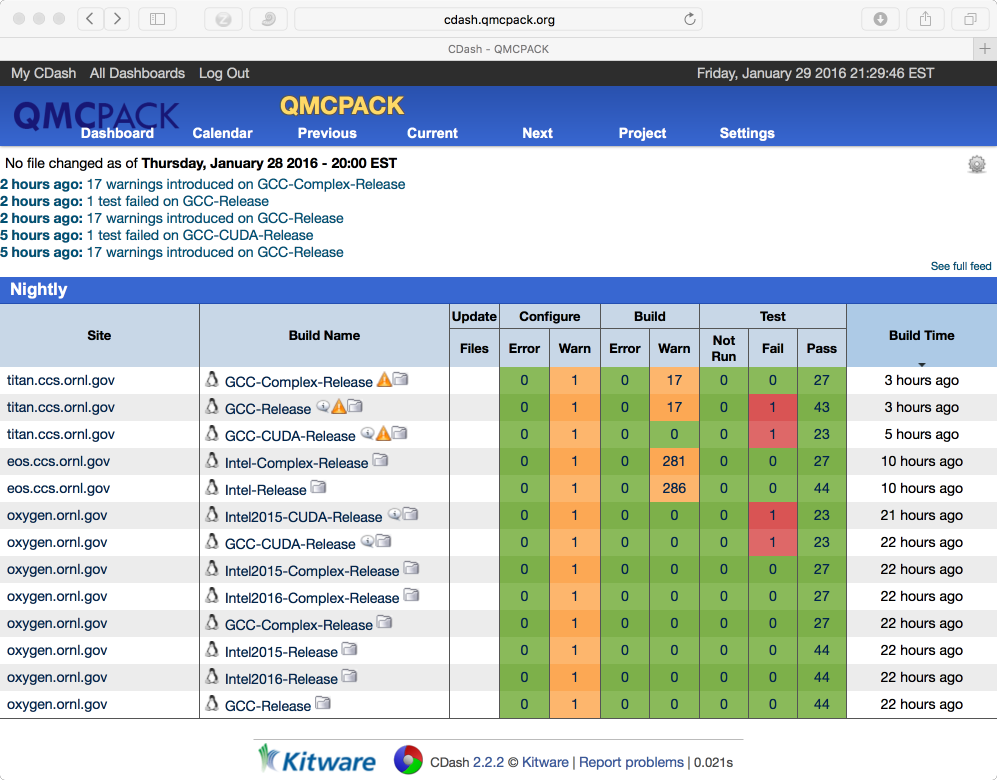
\includegraphics[width=10cm]{./figures/QMCPACK_CDash_CTest_Results_20160129.png}
  \caption{Example test results for QMCPACK showing data for a
    workstation (Intel, GCC, both CPU and GPU builds) and for two ORNL
    supercomputers. In this example, four errors were found. This
    dashboard is accessible at \url{https://cdash.qmcpack.org}.}
\end{figure}

\section{Building ppconvert, a pseudopotential format converter}
\label{sec:buildppconvert}
QMCPACK includes a utility---ppconvert---to convert between different
pseudopotential formats. Examples include effective core potential
formats (in Gaussians), the UPF format used by QE, and
the XML format used by QMCPACK itself. The utility also enables the
atomic orbitals to be recomputed via a numerical density functional
calculation if they need to be reconstructed for use in an
electronic structure calculation.

The utility is a stand-alone C++ executable that is not built by default but that is accessible via adding
\ishell{-DBUILD_PPCONVERT=1} to CMake and then typing \ishell{make ppconvert}.
A user guide is provided in Section~\ref{sec:ppconvert}.

\section{Installing and patching Quantum ESPRESSO}
\label{sec:buildqe}
For trial wavefunctions obtained in a plane-wave basis, we mainly
support QE. Note that ABINIT and QBox were supported historically
and could be reactivated.

QE stores wavefunctions in a nonstandard internal
``save'' format. To convert these to a conventional HDF5 format file
we have developed a converter---pw2qmcpack---which is an add-on to the
QE distribution.

To simplify the process of patching QE we have developed
a script that will automatically download and patch the source
code. The patches are specific to each version. For example, to download and
patch QE v6.3:

\begin{shade}
cd external_codes/quantum_espresso
./download_and_patch_qe6.3.sh
\end{shade}
After running the patch, you must configure QE with
the HDF5 capability enabled in either way:
\begin{itemize}
\item If your system already has HDF5 installed with Fortran, use the -{}-with-hdf5 configuration option.

\begin{shade}
cd qe-6.3
./configure --with-hdf5=/opt/local   # Specify HDF5 base directory
\end{shade}
   {\bf Check} the end of the configure output if HDF5 libraries are found properly.
   If not, either install a complete library or use the other scheme. If using a parallel HDF5 library, be sure to use
   the same MPI with QE as used to build the parallel HDF5 library.

   Currently, HDF5 support in QE itself is preliminary. To enable use of pw2qmcpack
   but use the old non-HDF5 I/O within QE, replace \ishell{-D__HDF5} with \ishell{-D__HDF5_C} in make.inc.
\item If your system has HDF5 with C only, manually edit make.inc by adding \ishell{-D__HDF5_C} and \ishell{-DH5_USE_16_API}
   in \ishell{DFLAGS} and provide include and library path in \ishell{IFLAGS} and \ishell{HDF5_LIB}.
\end{itemize}

The complete process is described in external\_codes/quantum\_espresso/README.

The tests involving pw.x and pw2qmcpack.x have been integrated into the test suite of QMCPACK.
By adding \ishell{-D QE_BIN=your_QE_binary_path} in the CMake command line when building your QMCPACK,
tests named with the ``qe-'' prefix will be included in the test set of your build.
You can test the whole pw $\to$ pw2qmcpack $\to$ qmcpack workflow by

\begin{shade}
ctest -R qe
\end{shade}
See Section~\ref{sec:integtestqe} and the testing section for more details.

\section{How to build the fastest executable version of QMCPACK}
\label{sec:buildperformance}
To build the fastest version of QMCPACK we recommend the following:
\begin{itemize}
\item Use the latest C++ compilers available for your
  system. Substantial gains have been made optimizing C++ in recent
  years.
\item Use a vendor-optimized BLAS library such as Intel MKL and AMD ACML. Although
  QMC does not make extensive use of linear algebra, it is used in the
  VMC wavefunction optimizer to apply the orbital coefficients in local basis
  calculations and in the Slater determinant update.
\item Use a vector math library such as Intel VML.  For periodic
  calculations, the calculation of the structure factor and Ewald
  potential benefit from vectorized evaluation of sin and
  cos. Currently we only autodetect Intel VML, as provided with MKL,
  but support for MASSV and AMD LibM is included via \#defines. See,
 for example, src/Numerics/e2iphi.h. For
  large supercells, this optimization can gain 10\% in performance.
\end{itemize}

Note that greater speedups of QMC calculations can usually be obtained by
carefully choosing the required statistics for each
investigation. That is, do not compute smaller error bars than necessary.

\section{Troubleshooting the installation}
\label{sec:troubleshoot}
Some tips to help troubleshoot installations of QMCPACK:
\begin{itemize}
\item First, build QMCPACK on a workstation you control or on any
  system with a simple and up-to-date set of development
  tools. You can compare the results of CMake and QMCPACK on this
  system with any more difficult systems you encounter.
\item Use up-to-date development software, particularly a recent
  CMake.
\item Verify that the compilers and libraries you expect are
  being configured. It is common to have multiple versions
  installed. The configure system will stop at the first version it
  finds, which might not be the most recent. If this occurs, directly specify the appropriate
  directories and files (Section
  \ref{sec:cmakeoptions}). For example, 
  \begin{shade}
  cmake -DCMAKE_C_COMPILER=/full/path/to/mpicc -DCMAKE_CXX_COMPILER=/full/path/to/mpicxx ..
  \end{shade}
\item To monitor the compiler and linker settings, use a verbose build, \ishell{make
  VERBOSE=1}. If an individual source file fails to compile you
  can experiment by hand using the output of the verbose build to
  reconstruct the full compilation line.
\end{itemize}

If you still have problems please post to the QMCPACK Google group with full
details, or contact a developer.
